% THIS IS AN EXAMPLE DOCUMENT FOR VLDB 2012
% based on ACM SIGPROC-SP.TEX VERSION 2.7
% Modified by  Gerald Weber <gerald@cs.auckland.ac.nz>
% Removed the requirement to include *bbl file in here. (AhmetSacan, Sep2012)
% Fixed the equation on page 3 to prevent line overflow. (AhmetSacan, Sep2012)

\documentclass{vldb}
\usepackage{graphicx}
\usepackage{color}
\usepackage{balance}  % for  \balance command ON LAST PAGE  (only there!)
\usepackage{times}
\usepackage{url}
\usepackage{algorithm}
\usepackage[noend]{algorithmic}
\usepackage{subfigure}
\usepackage{xspace}
\usepackage[noend]{algorithmic}
\usepackage{enumerate}
\usepackage{multirow}
\usepackage{epstopdf}
\usepackage{cleveref}
\newcommand{\squishlist}{
   \begin{list}{$\bullet$}
    {
      \setlength{\itemsep}{0pt}
      \setlength{\parsep}{3pt}
      \setlength{\topsep}{3pt}
      \setlength{\partopsep}{0pt}
      \setlength{\leftmargin}{1.5em}
      \setlength{\labelwidth}{1em}
      \setlength{\labelsep}{0.5em} } }

\newcommand{\squishend}{
    \end{list}  }

\newcommand{\argmax}{\operatornamewithlimits{arg\ max}}

\newcommand{\eat}[1]{}
\newcommand{\todo}[1]{\textcolor{red}{{TODO: #1}}}
\newcommand{\add}[1]{\textcolor{red}{{ADD: #1}}}
\newcommand{\note}[1]{\textcolor{blue}{{#1}}}

\newtheorem{definition}{Definition}
\newtheorem{example}{Example}
\newtheorem{theorem}{Theorem}
\newtheorem{lemma}{Lemma}
\newtheorem{problem}{Problem}
\newtheorem{reduction}{Reduction}
\newcommand{\domain}{\mathcal{D}}
\newcommand{\attributes}{\mathcal{A}_D}
\newcommand{\hierarchy}{\mathcal{H}_D}
\newcommand{\attrhierarchy}{\mathcal{H}_A}
\newcommand{\workers}{\mathcal{W}}
\newcommand{\uentities}{\mathcal{E}}
\newcommand{\queryvector}{{\bf Q_S}}



\begin{document}

% ****************** TITLE ****************************************

\title{CrowdGather: Budgeted Entity Extraction over Hierarchies}

\numberofauthors{3} 

\author{
}

\maketitle

\begin{abstract}

\end{abstract}




\section{Introduction}
Combining human computation with traditional computer systems has been recently proven beneficial in a growing number of complex application domains, including entity deduplication~\cite{wang:2012}, crowdsourced database systems~\cite{franklin:2011, marcus:2011}, knowledge base completion~\cite{kondredi:2014, west:2014}, entity extraction and structured data collection~\cite{trushkowsky:2013, park:2014}. 

We focus on the problem of using the crowd to extract entities from {\em structured domains}, i.e., domains that can be fully described by a collection of predicates following a pre-specified structure (e.g., a hierarchy), while adhering to constraints on the monetary cost and latency of the extraction process. Recently, Trushkowsky et al.~\cite{trushkowsky:2013} studied the problem of {\em crowdsourced entity extraction} in the context of crowdsourced databases focusing on the completeness and cost of the result for a specific enumeration query, where each query can be viewed as a single point of the entity domain. 
Often, however, applications require extracting entities over multiple domain points at the same time raising several challenges. Next, we use examples from two real-world scenarios to illustrate these challenges. 

%How crowd-sourcing can be used to enumerate entities. 

%Reasons why ``Getting it all" will not work

%Reasons why Hidden DBs approaches do not work

\subsection{Challenges}
\ \\Challeges
\begin{enumerate}
\item Limited budget - exploiting known hierarchies of entities to maximize extracted entities.
\item Extract the tail of the popularity distribution.
\item Estimating the unseen (i.e., how many new entities will we get with an extra query).
\item Dependent sampling in single and multiple hierarchies.
\end{enumerate}

The first scenario is that of collecting listings, such as business, job or event listings.

Challenges to discuss:
\begin{enumerate}
\item Show how one can guide workers to different points of the domain. Ideally, example to show that with the same number of queries we get more data.
\item Given a budget how to select which points of the domain to focus on.
\end{enumerate}

The second scenario is that of 


\subsection{Contribution}
\ \\Contributions
\begin{enumerate}
\item Introduce problem of budgeted entity enumeration.
\item How to exploit hierarchies to maximize/diversify the set of extracted entities under a budget constraint. Prove complexity of the problem. 
\item Estimators for calculating the number of new entities per query.
\item Estimators for dependent nodes, single and multiple hierarchies.
\item Heuristics, UCB style algorithms, with guarantees for independent nodes.
\item Experimental evaluation \textcolor{blue}{(NOTE: we need to think of baselines)}.
\end{enumerate}



\section{An Overview}
In this section we first review the problem of {\em crowdsourced entity extraction} and introduce a {\em budgeted} version of the basic problem. Then, we formally define the problem of {\em budgeted entity extraction over multiple hierarchies}, and finally, present an overview of our solution for the latter.

\subsection{Crowdsourced Entity Extraction}
%Present problem of crowdsourced entity enumeration. 
Let $\domain$ be a domain of entities that follows an open-world assumption, that is, incomplete or no information is available about which entities are contained in $\domain$. We assume knowledge of a set of discrete attributes $\attributes = \{A_1, A_2, \dots, A_d\}$ characterizing $\domain$. Let $dom(A_i)$ denote the domain of each attribute $A_i  \in \attributes$. Then, $\domain$ is the Cartesian product of $dom(A_1), \dots, dom(A_d)$. In the reminder of the paper we will refer to each element of the Cartesian product as a {\em point} in $\domain$, i.e., a point is a possible combination of values of all dimensions. We will also refer to a collection of points for which only a subset of attributes shares the same value as a {\em slice} of $\domain$. For example all points for which attribute $A_1 = x$ but all other attributes may take any value constitute a slice. 

The basic version of {\em crowdsourced entity extraction}~\cite{trushkowsky:2013} seeks to enumerate entities that belong in a single slice $\domain_P$ of $\domain$, specified by a set of predicates $P$ over a subset of attributes in $\attributes$. For example, consider the entity domain $\domain$ to be that of all ``Concerts" and the attributes describing the entities in $\domain$ to be $\attributes = \{$``Band Name", ``Location", ``Music Genre"$\}$. An instance of crowdsourced entity extraction corresponds to listing concerts with LOCATION = ``Boston, MA" and GENRE = ``Rock". 

We assume three different types of crowdsourced queries for answering an entity extraction problem as the one described above. The first type corresponds to {\em single entity queries} where workers are required to provide ``one more" entity that satisfies the query predicates. The second type of queries corresponds to {\em queries of  size k} where workers are asked to provide up to $k$ distinct entities. Finally, the last type corresponds to {\em exclude list queries}. Here,  workers are provided with $l$ entities that have already been extracted and are required to provide up to $k$ distinct entities under the constraint that none of them is included in the exclude list. It is easy to see that the last type of queries generalizes the previous two. Therefore, in the remainder of the paper, we will consider that all queries of the third type. To describe a query, we will use the notation $q(k,l)$ denoting a query of size $k$ accompanied with an exclude list of length $l$. 

Assuming an infinite pool of crowd workers,  one can extract entities satisfying a set of desired predicates by repeatedly asking workers queries with different configurations $q(k,l)$ across {\em multiple rounds}. However, in a typical crowdsourcing environment, tasks have different costs depending on their difficulty. Thus, crowdsourced queries of different difficulties should also exhibit different costs. Given a query $q(k,l)$, we assume that its cost is given by a function $c(\dot)$ with the following properties: (a) given an exclude list of fixed length $l$ then $c(q(k^{\prime},l)) \geq c(q(k,l)),  \forall k^{\prime} \geq k$, and (b) given a fixed query size $k$ then $c(q(k,l^{\prime})) \geq c(q(k,l)), \forall l^{\prime} \geq l$. 

The above naturally gives raise to a tradeoff between the total number of extracted entities and the total cost. Let $\pi$ denote a {\em querying policy}, that is, a chain of query configurations defining the crowdsourced queries issued at each round. Moreover, let $\uentities(\pi)$ be the total number of unique entities extracted following policy $\pi$ and $C(\pi)$ be the total cost of following querying policy $\pi$. Finally, we assume a monetary budget $\tau_c$ imposing a constraint on the total cost of a selected querying policy. We define the problem of budgeted crowdsourced entity extraction as follows:

\begin{definition}[Budgeted Entity Extraction]
Let $\domain$ be a given entity domain and $\tau_c$ a monetary budget on the total cost of issued queries. The Budgeted Entity Extraction problem seeks to find 
a querying policy $\pi^*$ that maximizes the number of unique entities extracted $\uentities(\pi^*)$ under the constraint $C(\pi^*) \leq \tau_c$.
\end{definition}

Measuring the effectiveness of different policies on extracting entities requires reasoning about the number of {\em new entities} returned by each query. In the remainder of the paper, we also refer to the number of new entities extracted by a query as the {\em return of the query}. The exact number of new entities returned by each query is unknown before issuing the query and thus one needs to estimated it using the expected number of new entities returned by a query $q(k,l)$. In their recent work, Trushkowsky et al.~\cite{trushkowsky:2013} showed how techniques from the species estimation literature can be used to estimate the new entities returned by queries of the form $q(1,0)$. Furthermore, the authors propose a {\em pay-as-you-go} scheme where one repeatedly issues $q(1,0)$ queries to the crowd until the {\em marginal gain}, i.e., the difference between the new extracted entities and the querying cost, drops below a desired threshold. However, the proposed scheme is agnostic to budget constraints as it does not enforces them explicitly. 


%\subsection{Budgeted Entity Extraction}
%
%We assume a monetary budget imposing a limitation on the total number of queries that can be issued to workers. Let $\mathcal{P}(\domain)$ denote a the possible slices of the domain $\domain$. Moreover, let $S \subseteq \mathcal{P}(\domain)$ be a subset of selected slices from $\mathcal{P}(\domain)$, and $\queryvector$ a vector containing the number of queries issued to workers for each element in $S$.  We denote with $\uentities(\queryvector)$ the total number of  unique entities extracted from the queries in $\queryvector$ and $C(\queryvector)$ the total cost  of the queries in $\queryvector$. We define the problem of budgeted crowdsourced entity extraction as follows:
%
%\begin{definition}[Budgeted Entity Extraction]
%Let $\domain$ be an entity domain, $\beta_c$ be a monetary budget on the total cost of issued queries. The Budgeted Entity Extraction problem seeks to find a subset $S \subseteq \mathcal{P}(\domain)$ and the corresponding query vector $\queryvector$ that maximizes the number of unique entities extracted  $\uentities(\queryvector)$ under the constraint $C(\queryvector) \leq \beta_c$.
%\end{definition}


%Using the technique proposed by Trushkowsky et al.~\cite{trushkowsky:2013} one can: (a) either iterate over all the points in $\domain$ or (b) consider $\domain$ as a single slice until the budget is exhausted  However, these two extreme approaches come with obvious limitations.
%
%The limitations of the first approach are rather obvious. First, the number of points in $\domain$ is exponentially large with respect to the number of attributes specifying the domain, and hence, for domains with a large number of attributes iterating over all points can be prohibitive given a budget constraint. Second, there might exist a large number of sparse or non-populated points in $\domain$.  
%
%To understand the limitations of the second approach,  we point out that crowdsourced entity extraction can be viewed as being equivalent to sampling items from a population with an unknown {\em popularity distribution}. The popularity distribution quantifies the probability of observing an item in a random sample from the underlying population. The efficiency of crowdsourced entity extraction is heavily affected by the popularity distribution characterizing the underlying domain~\cite{trushkowsky:2013}. Under skewed distributions one needs to issue a large number of queries to workers to obtain a sufficient coverage of the underlying entities. In cases where the domain contains a large number of entities, the cost of the queries might be prohibitive under the given budget. Moreover, due to the skew of the popularity distribution one may not be able to extract entities from slices of the domain $\domain$, whose entities belong in the tail of the distribution. Next, we focus on hierarchical domains and discuss how one can exploit their structure when solving the problem of crowdsourced budgeted entity extraction. 

\subsection{Extracting Entities over Hierarchies}
Next, we focus on structured domains where each attribute in $\attributes$ are hierarchically organized. For example, we consider the domain of  ``Concerts", where the attributes describing the underlying entities are $\attributes = \{$``Band Name", ``Location", ``Music Genre"$\}$. It is easy to see that the values for the attribute LOCATION, as well as the values for the attribute MUSIC GENRE are hierarchically organized. For example, location can simply refers to a country or a state in a country or even a city. When multiple hierarchies describe the entity domain, we consider a {\em unified hierarchy} corresponding to a lattice formed by taking the crossproduct of all available hierarchies. We denote this crossproduct as $\hierarchy$. 

Each node in $\hierarchy$ represents a slice of the data domain. Again, we assume a querying model as the one described before, however, we assume that queries can be issued at the level of nodes in $\hierarchy$. The basic definition of budgeted entity extraction can be extended for hierarchical domains as follows:
\begin{definition}[Hierarchical Entity Extraction]
Let $\domain$ be a hierarchical entity domain, described by a lattice $\hierarchy$, $\beta_c$ be a monetary budget on the total cost of issued queries. The Budgeted Hierarchical Entity Extraction problem seeks to find querying policy $\pi_S^*$ over a subset of nodes $S \subseteq \hierarchy$ that maximizes the number of unique entities extracted  $\uentities(\pi_S^*)$ under the constraint $C(\pi_S^*) \leq \tau_c$.
\end{definition}

Notice that apart from determining the right policy over the possible query configurations $q(k,l)$ we are also required to detect the optimal subset of nodes in $\hierarchy$ to be queried so that the total number of extracted entities is maximized under the given budget constraint. Clearly the problem of budgeted hierarchical entity extraction is a generalization of the first problem. However, the problem becomes more challenging as the number of nodes in $\hierarchy$ is exponential with respect to the number of attributes characterizing the domain under consideration. Moreover, queries across different nodes in $\hierarchy$ are not independent, hence, one needs to be able to updates the estimated return for a specific node in $\hierarchy$ considering indirect information obtained from querying nodes related to it.

%\ \\ \textbf{Single Hierarchy:}
%
%\ \\ \textbf{Multiple Hierarchies:}
%
%\ \\(1) Describe how domain changes when query nodes are connected via hierarchies. Present example. 
%
%\ \\(2) Discuss why cost may increase as we query nodes lower in the hierarchy (i.e., more specialized queries). Cost is a function of both monetary cost and latency.
%
%\ \\(3) Present optimization problem with hierarchies.

\subsection{Solution Overview}
We present an overview of our proposed framework for solving the problem of budgeted hierarchical entity extraction. We assume a large entity domain $\domain$ described by a set of attributes $\attributes$ with each attribute $A \in \attributes$ following a known hierarchy $\attrhierarchy$. One challenge in large entity domains is detecting parts of the domain with a small number of entities and avoid spending a the given budget on those. A fundamental idea to our framework is maximizing the number of extracted entities under the given budget by exploiting the structure of each $\attrhierarchy$, i.e., (a) the domain partitioning imposed by $\attrhierarchy$  and (b) the overlap of the hierarchy nodes. 


The problem of budgeted entity extraction can be viewed as an online optimization problem over multiple rounds, where at each round we seek to find the best query-node combination so that the total number of extracted entities over all rounds is maximized. An overview of the proposed framework is shown in \Cref{fig:framework}.

\begin{figure}
	\begin{center}
	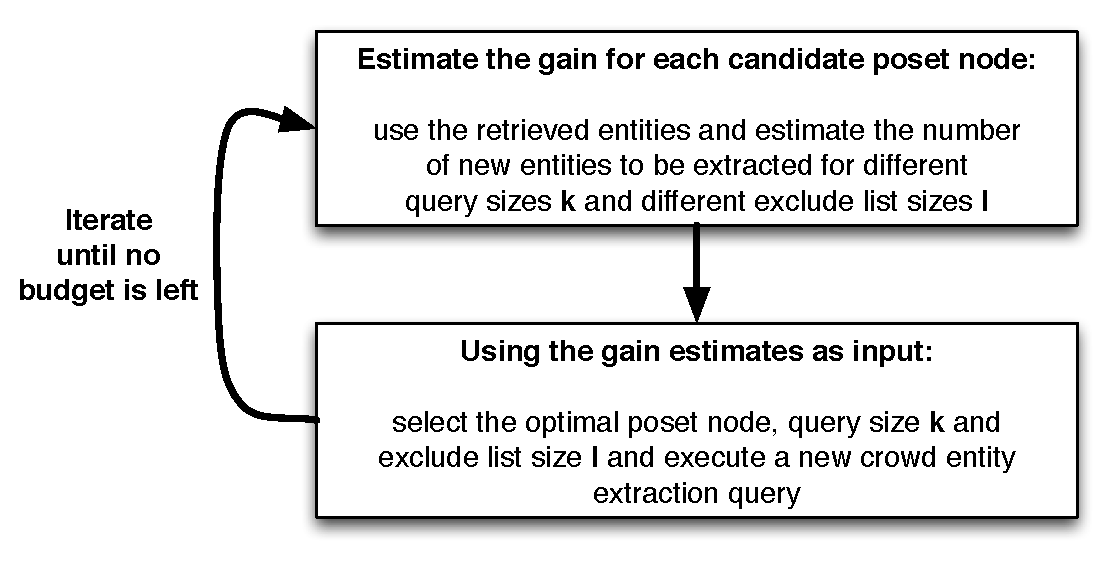
\includegraphics[clip,scale=0.5]{figs/framework.eps}
	\caption{Solution overview for budgeted entity extraction.}
	\label{fig:framework}
	\end{center}
\end{figure}

At a high-level, our solution consists of two major components. The first component is responsible for estimating the return obtained when an extra query $q(k,l)$ is issued at a certain node of $\hierarchy$. The second component takes as input the estimated returns for different nodes in the hierarchy and is responsible for finding the querying policy that will maximize the total return across all rounds under the specified budget constraints. We discuss the two components in \Cref{sec:estimation} and \Cref{sec:solution} respectively.  The following assumptions are made in the remainder of the paper:
\begin{itemize}
\item We assume that for each attribute $A \in \attributes$ the corresponding hierarchy $\attrhierarchy$ is known. 
\item We assume that after issuing a query we can associate each of the retrieved answers with all relevant nodes across all attribute hierarchies, i.e., a worker will provide all the attribute values describing a reported entity.
\end{itemize}

%At a high-level, our solution starts by selecting to query a node in $\hierarchy$ that maximizes the expected return, i.e., maximizes the difference between the {\em gain} from extracting entities and the {\em querying cost}. Then, depending on the retrieved entities, it selects one of the following actions: it (a) either continues querying the same node or (b) it selects to query a different node of similar level (i.e., different partitions of the entity domain) or (c) it progressively queries more specialized nodes originating from the current query node by traversing the hierarchy (\Cref{sec:solution}). This approach allows us to discover sparsely populated parts of the hierarchy in an online manner, and hence, limit the budget spent on them.
%
%The two main components of our approach are: (a) estimating the expected return for each available query node and (b) deciding which of the aforementioned actions to take. We discuss the two components in detail in \Cref{sec:estimation} and \Cref{sec:solution} respectively.  Finally, we make the following assumptions in the rest of the paper:
%\begin{itemize}
%\item We assume that the entire hierarchy describing the given entity domain is known. 
%\item We assume that after each query we can associate each of the retrieved answers with a leaf node in the hierarchy. In particular, we assume that a worker will provide all the attribute values describing a reported entity.
%\item Finally, we assume a fix type of queries that require each worker to provide us with a fixed number of unique entities per query. 
%\end{itemize}

%\ \\Give an overview of proposed solution
%\begin{enumerate}
%\item Input: Hierarchy, budget, cost per query.
%\item High-level description of online estimators. 
%\item Online optimization problem. 
%\end{enumerate}
%
%\ \\Clearly state and motivate the assumptions made throughout the paper
%\begin{enumerate}
%\item Entity hierarchies are known.
%\item Fixed query size (i.e., give me 5 more). Cost increases as we move to nodes lower in the hierarchy.
%\item After each query we can associate each of the answers with a leaf in the hierarchy. We assume full knowledge of all the attribute values of each entity.
%\end{enumerate}

\section{Estimating the Unseen Entities}
\label{sec:estimation}

%\textcolor{red}{Notes for this section:
%\squishlist
%\item Empirical estimates (extrapolation techniques) vs. chao based estimators
%\item Describe output of estimation component: Table N x C, where N corresponds to different nodes in the hierarchy, and C to different $q(k,l)$ query configurations
%\item Describe how to construct the exclude list, i.e., order items in decreasing order of appearance frequency and grab the top-$l$ items. 
%\item Came up with a new upper bound for the new number of items for different query sizes and different exclude list sizes. The upper bound combines extrapolation techniques with some of the tools used to derive the original Chao estimators. I need to test if the new upper bound is useful or not. 
%\item Bootstrapping to derive variance. 
%\item Consider if we should move away from purely empirical techniques and compare the new estimator with the standard Shen estimator. 
%\squishend}

The first component of our framework is responsible of estimating the number of new unique entities that will be extracted if a query $q(k,l)$ is issued at any node in $\hierarchy$.  
In this section we leverage techniques from the species estimation literature to solve the problem of estimating the return of a query $q(k,l)$ issued at any node in $\hierarchy$. We first show how the problem of estimating the return for queries of different sizes is equivalent to that of estimating the number of new species extracted by further sampling from an unknown population given a running sample~\cite{shen:2003}. In particular, we examine two techniques estimation techniques, one parametric and one non-parametric technique. Then, we show how the proposed techniques can be extended for scenarios where an {\em exclude list} is provided. An exclude list can be formally defined as a set of observed entities that are provided to workers during query time and correspond to invalid answers that should not be provided by the worker. 

\subsection{Query Return and Species Estimation}
One of the most important problems in the species estimation literature is that of predicting the number of new species in further sampling. More precisely, we assume an unknown population of species and an initial sample from that population of size $n$. Given this setup, our goal is to predict the number of new species that will be discovered in a new sample of size $m$. Similarly during hierarchical crowdsourced entity extraction we have an unknown population of entities and our goal is to extract distinct entities from it. Different nodes in the hierarchy cover different parts of the population. In general this parts can be overlapping. The results of each query at a specific node can be viewed as a sample from the population corresponding to that node. Given a number of previously executed queries, we have a sample of observed entities for a specific node in $\hierarchy$. As in further sampling we want to estimate the number of new entities extracted from a new sample of size $m$. Moreover, we want to consider a given exclude list of size $l$.

\subsection{A Regression Based Estimator}
We review an existing regression based estimator for the number of new entities for an increased query of some $m$. Let $n$ denote the existing sample size, $S$ the total number of entities present in the world, and $D_n$ the number of distinct entities in the sample. Finally, let $f_i$ denote the number of entities that appear $i$ times in the sample. To derive the new lower bound we make used of the generalized jackknife procedure for species richness estimation. Given two (biased) estimators of $S$, say $\hat{S}_1$ and $\hat{S}_2$, let $R$ be the ratio of their biases:
\begin{equation}
R = \frac{E(\hat{S}_1) - S}{E(\hat{S}_2) - S}
\end{equation}
By the generalized jackknife procedure, we can completely eliminate the estimating bias resulting from either $\hat{S}_1$ or $\hat{S}_2$ via
\begin{equation}
S = G(\hat{S}_1, \hat{S}_2) = \frac{\hat{S}_1 - R\hat{S}_2}{1 - R}
\label{eq:jknife}
\end{equation}
provided the ratio of biases is known. This is not true, and thus, we need to estimate $R$. 

We consider the following two biased estimators of $S$: $\hat{S_1} = D_n$ and $\hat{S}_2 = \sum_{j=1}^n D_{n-1}(j)/n = D_n - f_1/n$ where $D_{n-1}(j)$ is the number of species discovered with the $j$th observation removed from the original sample. Replacing these estimators in \Cref{eq:jknife} gives us:
\begin{equation}
S = D_n +\frac{R}{1-R}\frac{f_1}{n}
\end{equation}

Similarly, for a sample of increased size $n+m$ we have:
\begin{equation}
S = D_{n+m} +\frac{R^{\prime}}{1-R^{\prime}}\frac{f^{\prime}_1}{n+m}
\end{equation}
where $R^{\prime}$ is the ratio of the biases and $f^{\prime}_1$ the number of singleton entities for the increased sample.

Let $K = \frac{R}{1-R}$ and $K^{\prime} = \frac{R^{\prime}}{1-R^{\prime}}$. Taking the difference of the previous two equations we have:
\begin{equation}
D_{n+m} - D_{n} = K\frac{f_1}{n} - K^{\prime}\frac{f^{\prime}_1}{n+m}
\end{equation}

Therefore, we have:
\begin{equation}
\label{eq:new}
new = K\frac{f_1}{n} - K^{\prime}\frac{f^{\prime}_1}{n+m}
\end{equation}

We need to estimate $K$, $K^{\prime}$ and $f^{\prime}_1$. We start with $f^{\prime}_1$ denoting the number of singleton in the increased sample of size $n+m$. Notice, that $f^{\prime}_1$ is not known since we have not obtained the increased sample yet, so we need to express it in terms of $f_1$, i.e., the number of singletons, in the running sample of size $n$. We have:
\begin{equation}
f^{\prime}_1 = new + f_1 - f_1*\Pr[\mbox{in query of size m}]
\end{equation}
Following an approach similar to Shen et al.~\cite{shen:2003}, we have that the probability of a singleton appearing in a query of size $m$ is:
\begin{equation}
\Pr[\mbox{in query of size m}] = \sum_{k=0}^m(1-(1-\frac{1}{f_1})^k) {m \choose k}(1-p_1)^k p_1^{m-k}
\end{equation}
where $p_1$ denotes the probability that a singleton item in the sample of size $n$ will be selected in a future query. We estimate this probability using the corresponding Good-Turing estimator considering the running sample. We have:
\begin{equation}
p_1 = \hat{\theta}(1) = \frac{1}{n}2\frac{N_2}{N_1}
\end{equation} 
where $N_2$ is the number of entities that appear twice in the sample and $N_1$ is the number of singletons. 
Eventually we have that:
\begin{align}
f^{\prime}_1 &= new + f_1(1- \sum_{k=0}^m(1-(1-\frac{1}{f_1})^k) {m \choose k}(1-p_1)^k p_1^{m-k}) \nonumber \\
f^{\prime}_1 &= new + f_1(1- P)
\end{align}
Replacing the last equation in \Cref{eq:new} we have:
\begin{align}
&new = K\frac{f_1}{n} - K^{\prime}\frac{new + f_1(1- P)}{n+m} \nonumber \\
&new = K\frac{f_1}{n} - K^{\prime}\frac{new}{n+m} - K^{\prime}\frac{f_1(1- P)}{n+m} \nonumber \\
&new(1 + \frac{K^{\prime}}{n+m}) = K\frac{f_1}{n} - K^{\prime}\frac{f_1(1- P)}{n+m} \nonumber \\
&new = \frac{1}{(1 + \frac{K^{\prime}}{n+m})}(K\frac{f_1}{n} - K^{\prime}\frac{f_1(1- P)}{n+m}) \nonumber
\end{align}

Next, we discuss how one can estimate $K$ and $K_{\prime}$. To estimate $K$ we follow the extrapolation approach introduced by Hwang and Shen~\cite{hwang:2010}. Namely, from the Cauchy-Schwarz inequality we have that:
\begin{equation}
K = \frac{\sum_{i=1}^S (1-p_i)^n}{\sum_{i=1}^S p_i(1-p_i)^{n-1}} \geq \frac{(n-1)f_1}{2f_2}
\end{equation}
This can be generalized to:
\begin{equation}
K=\frac{nf_0}{f_1} \geq \frac{(n-1)f_1}{2f_2} \geq \frac{(n-2)f_2}{3f_3} \geq \dots
\end{equation}
Let $g(i) = \frac{(n-i)f_i}{(i+1)f_{i+1}}$. From the above we have that the function $g(x)$ is a smooth monotone function for all $x \geq 0$. Moreover, let $y_i$ denote a realization of $g(i)$ mixed with a random error. Hwang and Shen how one can use an exponential regression model to estimate $K$. The proposed model corresponds to:
\begin{equation}
y_i = \beta_0\exp(\beta_1i^{\beta_2}) + \epsilon_i
\end{equation}
where $i = 1, \dots, n-1$, $\beta_0 > 0$, $\beta_1 < 0$, $\beta_2 >0$ and $\epsilon_i$ denotes random errors. It follows that $K = \beta_0$. 

Finally, we show how one can estimate the value of $K_\prime$ for an increased sample of size $n+m$. First, we show that $K$ increases monotonically as the size of the running sample increases. Let $K(n) = \frac{\sum_{i=1}^S (1-p_i)^n}{\sum_{i=1}^S p_i(1-p_i)^{n-1}}$ be a function returning the value of $K$ for a sample of size $n$. We have the following lemma. 

\begin{lemma}
We have $K(n+m) \geq K(n), \forall n,m > 0$.
\end{lemma}
\begin{proof}
In the remainder of the proof we will denote $K(n+m)$ as $K^{\prime}$. By definition we have that $K = \frac{\sum_{i=1}^S (1-p_i)^n}{\sum_{i=1}^S p_i(1-p_i)^{n-1}}$ and $K^{\prime} = \frac{\sum_{i=1}^S (1-p_i)^{n+m}}{\sum_{i=1}^S p_i(1-p_i)^{n+m-1}}$. We want to show that:
{\small
\begin{align}
&\frac{\sum_{i=1}^S (1-p_i)^{n+m}}{\sum_{i=1}^S p_i(1-p_i)^{n+m-1}} \geq \frac{\sum_{i=1}^S (1-p_i)^n}{\sum_{i=1}^S p_i(1-p_i)^{n-1}} \nonumber \\
&\sum_{i=1}^S (1-p_i)^{n+m}\sum_{j=1}^S p_j(1-p_j)^{n-1} \geq \sum_{i=1}^S p_i(1-p_i)^{n+m-1}\sum_{j=1}^S (1-p_j)^n\nonumber \\
&\sum_{i,j:i\prec j}[(1-p_i)^{n+m}p_j(1-p_j)^{n-1} - p_i(1-p_i)^{n+m-1}(1-p_j)^n + \nonumber \\
& + (1-p_j)^{n+m}p_i(1-p_i)^{n-1} - p_j(1-p_j)^{n+m-1}(1-p_i)^n] \geq 0 \nonumber \\
&\sum_{i,j:i\prec j}[(1-p_i)^{n}(1-p_j)^{n-1}p_j((1-p_i)^{m} - (1-p_j)^{m})  + \nonumber \\
& - (1-p_j)^{n}p_i(1-p_i)^{n-1}((1-p_i)^{m} - (1-p_j)^{m}) \geq 0 \nonumber \\
&\sum_{i,j:i\prec j}[(1-p_i)^{n-1}(1-p_j)^{n-1}(p_j-p_i)((1-p_i)^{m} - (1-p_j)^{m}) \geq 0
\end{align}}

But the last inequality always holds since each term of the summation is positive. In particular, if $p_j \geq p_i$ then
also $1-p_i \geq 1-p_j$ and if $p_j \leq p_i$ then $1-p_i \leq 1-p_j$.
\end{proof}

We have that $K(n)$ is an increasing function of the sample size. Moreover, $K(n)$ has a decreasing slope. We model $K$ as a generalized logistic function of the form $f(x) = \frac{A}{1+exp(-G(x-D))}$. As we observe samples of different sizes for different queries we estimate $K$ as described above and therefore we observe different realizations of $f(\cdot)$. Thus, we can learn the parameters of $f$ and use it to estimate $K^{\prime}$.

\textcolor{red}{
\squishlist
\item extend estimator for exclude lists of different sizes. Simply construct the exclude list and remove the items in it from the running sample. 
\squishend
}

Maximizing the number of extracted entities in an online fashion requires estimating the expected return for each of the available query nodes. Assuming a known query cost and the current number of received entities for each node in $\hierarchy$,  this problem is equivalent that of estimating the number of new entities retrieved if we choose to query a certain node in the hierarchy. We distinguish between the two scenarios below:

\vspace{5pt}\noindent \textbf{Querying and estimating for the same node:}
We consider a certain node $q \in \hierarchy$, and assume that we have issued $t$ entity extraction queries for this node. Let $r_1, r_2, r_3, \dots, r_t$ denote the number of new distinct entities returned by each of the $t$ queries.  We wish to estimate the return of asking an extra query at node $x$, i.e, the value of $r_{t+1}$. To estimate this value we use an autoregressive model taking as input the values $r_1, r_2, \dots, r_t$. We observe that using such a model, we can predict the number of new distinct entities effectively due to the non-increasing trend of the value of newly observed entities. \note{NOTE: elaborate more on this. Point to emphasize: the return follows a non-increasing trend because (a) the number of new entities is upper bounded due to the query size and (b) it is affected by the popularity distribution.}

\vspace{5pt}\noindent \textbf{Querying and estimating for different nodes:} Due to the hierarchical structure of the entity domain we can obtain indirect information about the entities contained in nodes that were not queried explicitly. For example, when we query a node $q \in \hierarchy$ we also obtain information about the entities contained in its children. In general, when querying a node $q \in \hierarchy$ we obtain partial information about all the entities contained in other nodes that cover the same leaf nodes as $q$. We will refer to all these nodes as {\em dependent} nodes. More formally we have:

\begin{definition}[Dependent Node Set]
Let $\domain$ be an entity domain and $\hierarchy$ the hierarchy describing each structure. With $L(q)$ denoting the leaf nodes of $\hierarchy$ covered by a node $q \in \hierarchy$, we define the set of {\em dependent} nodes of $q$ to be the set of nodes $M(q) \subseteq \hierarchy \setminus \{q\}$ such that $\forall q^{\prime} \in M(q), L(q) \cap L(q^{\prime}) \neq \emptyset$.
\end{definition}

We leverage techniques from the species estimation literature to estimate the expected number of new entities returned when we choose to query a node for which only indirect information is available. Shen et al.~\cite{shen:2003}, derive an estimator for the number of new species $\hat{N}_{Shen}$ that would be found in an increased sample of size $m$. The approach assumes we have an estimate of the number of unobserved elements $\hat{f}_0$ and that the unobserved elements have equal relative abundances. Let $n$ denote the size of the running sample, $f_1$ the number of singletons in the running sample, $\hat{C} = 1 - \frac{f_1}{n}$ be the Good-Turing estimator of the coverage of the existing retrieved sample and $\hat{f}_0$ be an estimate on the number of unseen species.  An estimate of the unique elements found in an increased sample of size $m$ is given by:
\begin{equation}
\hat{N}_{Shen} = \hat{f}_0 \left( 1 - \left(1 - \frac{1 - \hat{C}}{\hat{f}_0}\right)^m\right)
\end{equation}

\note{NOTE: This probability is an upper bound}

\note{NOTE: Basic difference from getting it all paper} When we issue queries of the type ``give me k more items" we are basically performing sampling without replacement from the underlying population. Under such scenarios the Chao92 estimate used by Trushkowsky et al.~\cite{trushkowsky:2013} for the pay-as-you-go model will not be effective. However, Chao et al.~\cite{chao:2012} propose an estimate for $\hat{f}_0$ when sampling is done without replacement. Let $n$ be the total size of the running sample, $N$ the size of the underlying population and $q = n/N$, the estimate for the undetected species $\hat{f_0}$ is:
\begin{equation}
\hat{f}_0 = \frac{f_1^2}{2wf_2 + rf_1}
\end{equation}
where $w = n/(n-1)$ and $r = q/(1-q)$.
When $q \rightarrow 0$, i.e., the sample percentage is small, the above estimator is equivalent to the Chao1 estimator $\hat{f}_0 = \frac{n-1}{n} \frac{f_1^2}{2f_2}$.
Notice that we need to now the size of the underlying population to compute $q$. While this is not realistic for many applications, we can obtain an upper bound on the size of the population we expect to extract by exploiting the known budget constraint. From the two approaches described above we have an estimate for the return for both nodes that are queried directly and nodes that are queried indirectly. 

%\ \\(1) Focus on single node. Right now we have an ARIMA model for estimating the number of new entities for a single node. It comes without theoretical guarantees but we found it to be quite accurate. 
%\textcolor{red}{TODO: Extend current estimator to take multiple variables as input, i.e., size of current sample, number of unique entities, exclude list.}
%
%\ \\(2) \textcolor{red}{TODO: Design new estimator when entities from a node are sampled indirectly. Dependent sampling between parents and children in single hierarchy, nodes with overlapping entities in multiple hierarchies.}

\section{Solving Budgeted Entity Extraction}
\label{sec:solution}
\textcolor{red}{Notes for this section:
\squishlist
\item Clearly describe the challenges of this component. Number of  nodes in the hierarchy is huge, introduce myopic approach based on active frontier. 
\item Describe how budgeted hierarchical entity extraction corresponds to a combinatorial bandit optimization problem. Under this setup, we have certain ``super-arms" that consist of multiple simple arms. The rewards for the simple arms can be dependent. 
\item How can we propagate the variances of children to the variances of parents. 
\item Analyze the regret for the case of partitioning, single hierarchy, multiple hierarchies.
\squishend}
\subsection{Algorithmic Framework}

{
\small{
\begin{algorithm}[h]
\caption{Hierarchical Entity Extraction}
\begin{algorithmic}[1]
\STATE {\bf Input:} $\hierarchy$: the hierarchy describing the entity domain; $f$: value oracle access to benefit function; $\beta_c$: query budget;
\STATE {\bf Output:} $\uentities$: a set of extracted distinct entities;
\STATE $\uentities \leftarrow \{\}$
\STATE $QF \leftarrow \{\mbox{First level nodes of }\hierarchy\}$ /* Set query frontier */
\STATE $VQ \leftarrow \{\}$ /* Set visited queries */
\STATE $RB \leftarrow \beta_c$ /* Set remaining budget frontier */
\WHILE {$RB > 0$ and $QF \neq \{\}$}
	\STATE $\bar{w} \leftarrow <f(q)>_{q \in QF}$ /*Benefit vector of nodes in QF*/
	\STATE Sample a node $q$ to be queried using weights $\bar{w}$
	\WHILE {true}
		\STATE $E \leftarrow$ get more entities by querying node $q$; 
		\STATE $\uentities \leftarrow \uentities \cup E$ /* Update unique entities */
		\STATE $RB \leftarrow RB - C(q)$ /* Update budget */
		\STATE Update entity frequency estimates for $q$ and dependent nodes $M(q)$
		\STATE /* Decide if we need to stop querying q */
		\STATE $q^{\prime} \leftarrow \argmax_{x \in QF \cup M(q)} (f(x))$
		\IF {$q \neq q^{\prime}$}
			\STATE break
		\ENDIF
	\ENDWHILE
	\STATE $VS \leftarrow VS \cup \{q\}$
	\STATE $QF \leftarrow QF \cup M(q) \setminus VS$ /* Update query frontier */
\ENDWHILE
\RETURN $\uentities$
\end{algorithmic}
\end{algorithm}
}
}

\subsection{Analysis}
\ \\(1) Present basic UCB style heuristic for independent nodes. This version corresponds to the case where we have multiple non-overlapping partitions of the domain of interest. Present theoretical guarantees. 

\ \\(2) Heuristics for single hierarchy. Start from the top and work your way down the hierarchy. Actions per node: (a) continue querying, (b) stop querying the node and move to one of its children. 

\ \\(3) \textcolor{red}{TODO: Algorithm for multiple hierarchies.}

\ \\(4) \textcolor{red}{TODO: Extension of all algorithms to take into account an exclude list.}

\section{Experimental Evaluation}

\ \\\textcolor{red}{TODO: design experiments. What datasets shall we use? How to design real crowdsourcing experiments? Shall we evaluate the algorithm on a dataset similar to the Yelp dataset we have?}

\section{Related Work}
\ \\(1) Discuss ``Crowdsourcing enumeration queries". Present clearly why our work is different. 

\ \\(2) Discuss papers on species estimators.

\ \\(3) Briefly discuss related crowdsourcing work with budget and latency constraints.

\ \\(4) \textcolor{blue}{NOTE: Other papers?}


\section{Conclusion}


\bibliographystyle{abbrv}
\bibliography{crowd_hierarchies}

\begin{appendix}
\section{Derivation of new estimator}
We present a novel lower bound for the number of new entities for an increased query of some $m$. Let $n$ denote the existing sample size, $S$ the total number of entities present in the world, and $D_n$ the number of distinct entities in the sample. Finally, let $f_i$ denote the number of entities that appear $i$ times in the sample. To derive the new lower bound we make used of the generalized jackknife procedure for species richness estimation. Given two (biased) estimators of $S$, say $\hat{S}_1$ and $\hat{S}_2$, let $R$ be the ratio of their biases:
\begin{equation}
R = \frac{E(\hat{S}_1) - S}{E(\hat{S}_2) - S}
\end{equation}
By the generalized jackknife procedure, we can completely eliminate the estimating bias resulting from either $\hat{S}_1$ or $\hat{S}_2$ via
\begin{equation}
S = G(\hat{S}_1, \hat{S}_2) = \frac{\hat{S}_1 - R\hat{S}_2}{1 - R}
\label{eq:jknife}
\end{equation}
provided the ratio of biases is known. This is not true, and thus, we need to estimate $R$. 

We consider the following two biased estimators of $S$: $\hat{S_1} = D_n$ and $\hat{S}_2 = \sum_{j=1}^n D_{n-1}(j)/n = D_n - f_1/n$ where $D_{n-1}(j)$ is the number of species discovered with the $j$th observation removed from the original sample. Replacing these estimators in \Cref{eq:jknife} gives us:
\begin{equation}
S = D_n +\frac{R}{1-R}\frac{f_1}{n}
\end{equation}

Similarly, for a sample of increased size $n+m$ we have:
\begin{equation}
S = D_{n+m} +\frac{R^{\prime}}{1-R^{\prime}}\frac{f^{\prime}_1}{n+m}
\end{equation}
where $R^{\prime}$ is the ratio of the biases and $f^{\prime}_1$ the number of singleton entities for the increased sample.

Let $K = \frac{R}{1-R}$ and $K^{\prime} = \frac{R^{\prime}}{1-R^{\prime}}$. Taking the difference of the previous two equations we have:
\begin{equation}
D_{n+m} - D_{n} = K\frac{f_1}{n} - K^{\prime}\frac{f^{\prime}_1}{n+m}
\end{equation}

Therefore, we have:
\begin{equation}
\label{eq:new}
new = K\frac{f_1}{n} - K^{\prime}\frac{f^{\prime}_1}{n+m}
\end{equation}

We need to estimate $K$, $K^{\prime}$ and $f^{\prime}_1$. We start with $f^{\prime}_1$ denoting the number of singleton in the increased sample of size $n+m$. Notice, that $f^{\prime}_1$ is not known since we have not obtained the increased sample yet, so we need to express it in terms of $f_1$, i.e., the number of singletons, in the running sample of size $n$. We have:
\begin{equation}
f^{\prime}_1 = new + f_1 - f_1*\Pr[\mbox{in query of size m}]
\end{equation}
Following an approach similar to Shen et al.~\cite{shen:2003}, we have that the probability of a singleton appearing in a query of size $m$ is:
\begin{equation}
\Pr[\mbox{in query of size m}] = \sum_{k=0}^m(1-(1-\frac{1}{f_1})^k) {m \choose k}(1-p_1)^k p_1^{m-k}
\end{equation}
where $p_1$ denotes the probability that a singleton item in the sample of size $n$ will be selected in a future query. We estimate this probability using the corresponding Good-Turing estimator considering the running sample. We have:
\begin{equation}
p_1 = \hat{\theta}(1) = \frac{1}{n}2\frac{N_2}{N_1}
\end{equation} 
where $N_2$ is the number of entities that appear twice in the sample and $N_1$ is the number of singletons. 
Eventually we have that:
\begin{align}
f^{\prime}_1 &= new + f_1(1- \sum_{k=0}^m(1-(1-\frac{1}{f_1})^k) {m \choose k}(1-p_1)^k p_1^{m-k}) \nonumber \\
f^{\prime}_1 &= new + f_1(1- P)
\end{align}
Replacing the last equation in \Cref{eq:new} we have:
\begin{align}
&new = K\frac{f_1}{n} - K^{\prime}\frac{new + f_1(1- P)}{n+m} \nonumber \\
&new = K\frac{f_1}{n} - K^{\prime}\frac{new}{n+m} - K^{\prime}\frac{f_1(1- P)}{n+m} \nonumber \\
&new(1 + \frac{K^{\prime}}{n+m}) = K\frac{f_1}{n} - K^{\prime}\frac{f_1(1- P)}{n+m} \nonumber \\
&new = \frac{1}{(1 + \frac{K^{\prime}}{n+m})}(K\frac{f_1}{n} - K^{\prime}\frac{f_1(1- P)}{n+m}) \nonumber
\end{align}

Next, we discuss how one can estimate $K$ and $K_{\prime}$. To estimate $K$ we follow the extrapolation approach introduced by Hwang and Shen~\cite{hwang:2010}. Namely, from the Cauchy-Schwarz inequality we have that:
\begin{equation}
K = \frac{\sum_{i=1}^S (1-p_i)^n}{\sum_{i=1}^S p_i(1-p_i)^{n-1}} \geq \frac{(n-1)f_1}{2f_2}
\end{equation}
This can be generalized to:
\begin{equation}
K=\frac{nf_0}{f_1} \geq \frac{(n-1)f_1}{2f_2} \geq \frac{(n-2)f_2}{3f_3} \geq \dots
\end{equation}
Let $g(i) = \frac{(n-i)f_i}{(i+1)f_{i+1}}$. From the above we have that the function $g(x)$ is a smooth monotone function for all $x \geq 0$. Moreover, let $y_i$ denote a realization of $g(i)$ mixed with a random error. Hwang and Shen how one can use an exponential regression model to estimate $K$. The proposed model corresponds to:
\begin{equation}
y_i = \beta_0\exp(\beta_1i^{\beta_2}) + \epsilon_i
\end{equation}
where $i = 1, \dots, n-1$, $\beta_0 > 0$, $\beta_1 < 0$, $\beta_2 >0$ and $\epsilon_i$ denotes random errors. It follows that $K = \beta_0$. 

Finally, we show how one can estimate the value of $K_\prime$ for an increased sample of size $n+m$. First, we show that $K$ increases monotonically as the size of the running sample increases. Let $K(n) = \frac{\sum_{i=1}^S (1-p_i)^n}{\sum_{i=1}^S p_i(1-p_i)^{n-1}}$ be a function returning the value of $K$ for a sample of size $n$. We have the following lemma. 

\begin{lemma}
We have $K(n+m) \geq K(n), \forall n,m > 0$.
\end{lemma}
\begin{proof}
In the remainder of the proof we will denote $K(n+m)$ as $K^{\prime}$. By definition we have that $K = \frac{\sum_{i=1}^S (1-p_i)^n}{\sum_{i=1}^S p_i(1-p_i)^{n-1}}$ and $K^{\prime} = \frac{\sum_{i=1}^S (1-p_i)^{n+m}}{\sum_{i=1}^S p_i(1-p_i)^{n+m-1}}$. We want to show that:
{\small
\begin{align}
&\frac{\sum_{i=1}^S (1-p_i)^{n+m}}{\sum_{i=1}^S p_i(1-p_i)^{n+m-1}} \geq \frac{\sum_{i=1}^S (1-p_i)^n}{\sum_{i=1}^S p_i(1-p_i)^{n-1}} \nonumber \\
&\sum_{i=1}^S (1-p_i)^{n+m}\sum_{j=1}^S p_j(1-p_j)^{n-1} \geq \sum_{i=1}^S p_i(1-p_i)^{n+m-1}\sum_{j=1}^S (1-p_j)^n\nonumber \\
&\sum_{i,j:i\prec j}[(1-p_i)^{n+m}p_j(1-p_j)^{n-1} - p_i(1-p_i)^{n+m-1}(1-p_j)^n + \nonumber \\
& + (1-p_j)^{n+m}p_i(1-p_i)^{n-1} - p_j(1-p_j)^{n+m-1}(1-p_i)^n] \geq 0 \nonumber \\
&\sum_{i,j:i\prec j}[(1-p_i)^{n}(1-p_j)^{n-1}p_j((1-p_i)^{m} - (1-p_j)^{m})  + \nonumber \\
& - (1-p_j)^{n}p_i(1-p_i)^{n-1}((1-p_i)^{m} - (1-p_j)^{m}) \geq 0 \nonumber \\
&\sum_{i,j:i\prec j}[(1-p_i)^{n-1}(1-p_j)^{n-1}(p_j-p_i)((1-p_i)^{m} - (1-p_j)^{m}) \geq 0
\end{align}}

But the last inequality always holds since each term of the summation is positive. In particular, if $p_j \geq p_i$ then
also $1-p_i \geq 1-p_j$ and if $p_j \leq p_i$ then $1-p_i \leq 1-p_j$.
\end{proof}

We have that $K(n)$ is an increasing function of the sample size. Moreover, $K(n)$ has a decreasing slope. We model $K$ as a generalized logistic function of the form $f(x) = \frac{A}{1+exp(-G(x-D))}$. As we observe samples of different sizes for different queries we estimate $K$ as described above and therefore we observe different realizations of $f(\cdot)$. Thus, we can learn the parameters of $f$ and use it to estimate $K^{\prime}$.
\end{appendix}
\end{document}
